%% 이 파일은 서울대학교 산업공학과 학위논문 양식을 정의하기 위해 아래 원저자와 1차 수정자가 
%% 수정한 파일을 서울대학교 산업공학과에서 재수정하여 만든 파일입니다. (2018년 4월)
%% 원저자: zeta709 (zeta709@gmail.com) 
%% 1차 수정자: 서울대학교 데이터마이닝연구실 
\RequirePackage{fix-cm} 

% 옵션 수정 가능 
% oneside/twoside : 단면 인쇄, 양면 인쇄 
% openright : 챕터가 홀수쪽에서 시작
% draft, final,etc....
\documentclass[oneside, ko,ms]{snuthesis_utf8_kor}

%%%%%%%%%%%%%%%%%%%%%%%%%%%%%%%%%%%%%%%%
%% 목차 양식을 변경하는 코드
%% subfigure (subfig) package 사용 여부에 따라
%% tocloft의 옵션을 다르게 지정해야 한다.
%\usepackage[titles,subfigure]{tocloft} % when you use subfigure package
\usepackage[titles]{tocloft} % when you don't use subfigure package
%\usepackage{subfig}
\usepackage{amsmath,amssymb,amsthm,kotex,color}
%\usepackage[]{algorithm2e}
\usepackage{tikz}
\usetikzlibrary{shapes,arrows}
\usepackage[]{algpseudocode,algorithm,algorithmicx}
\usepackage{setspace}
\usepackage{array}
\usepackage{romanbar}
\usepackage{pgfplots}
\usepackage{caption}
\usepackage{subcaption}
\usepackage{booktabs, multirow}
\usepackage{threeparttable}
\usepackage{multirow}
\usepackage{rotating}
\usepackage{comment}
%\usepackage{indentfirst}\setlength\parindent{2em}

\makeatletter % don't delete me
\renewcommand\cftchappresnum{제 ~}
\renewcommand\cftchapaftersnum{ ~ 장}
\renewcommand\cftfigpresnum{그림 ~}
\renewcommand\cfttabpresnum{표 ~}
\renewcommand{\algorithmicforall}{\textbf{foreach}}

\newtheorem{theorem}{Theorem}[chapter]
\newtheorem{lemma}[theorem]{Lemma}
\newtheorem{proposition}[theorem]{Proposition}
\newtheorem{corollary}[theorem]{Corollary}
\newtheorem{definition}[theorem]{Definition}
\newtheorem{Proposition}{Proposition}
\newtheorem{remark}{Remark}[chapter]
\newtheorem{example}{Example}[chapter]
\usepackage[pdftex,bookmarks=true]{hyperref}

\makeatother % don't delete me
\newlength{\mytmplen}
\settowidth{\mytmplen}{\bfseries\cftchappresnum\cftchapaftersnum}
\addtolength{\cftchapnumwidth}{\mytmplen}
\settowidth{\mytmplen}{\bfseries\cftfigpresnum\cftfigaftersnum}
\addtolength{\cftfignumwidth}{\mytmplen}
\settowidth{\mytmplen}{\bfseries\cfttabpresnum\cfttabaftersnum}
\addtolength{\cfttabnumwidth}{\mytmplen}
%% 목차 양식을 변경하는 코드 끝
%%%%%%%%%%%%%%%%%%%%%%%%%%%%%%%%%%%%%%%%
%%%%%%%%%%%%%%%%%%%%%%%%%%%%%%%%%%%%%%%%
%% 다른 패키지 로드
%% http://faq.ktug.or.kr/faq/pdflatex%B0%FAlatex%B5%BF%BD%C3%BB%E7%BF%EB
%% 필요에 따라 직접 수정 필요
\ifpdf
	% \input glyphtounicode\pdfgentounicode=1 %type 1 font사용시
	%\usepackage[pdftex,unicode]{hyperref} % delete me
	%\usepackage[pdftex]{graphicx}
	%\usepackage[pdftex,svgnames]{xcolor}
\else
	%\usepackage[dvipdfmx,unicode]{hyperref} % delete me%
	%\usepackage[dvipdfmx]{graphicx}
	%\usepackage[dvipdfmx,svgnames]{xcolor}
\fi
%%%%%%%%%%%%%%%%%%%%%%%%%%%%%%%%%%%%%%%%
%
%% \title : 22pt로 나오는 큰 제목
%% \title*: 16pt로 나오는 작은 제목

\title{생산 계획 문제 해결을 위한 최적화 기법}
\title*{Mathematical Optimization Approaches for Solving Production Planning Problems}
\titlen{Mathematical Optimization Approaches for Solving Production Planning Problems}

\author{Gildong Hong}
\author*{홍길동} % Same as \author.
\authorn{홍~길~동}
\phonenumber{010-1234-1234}
\studentnumber{2018-12345}
\advisor{이지도}
\advisor*{Advisor~Lee}
\advisorn{이~지~도}
\graddate{2019~년~~2~월}
\submissiondate{2018~년~~11~월}
\submissiondaten{2018~년~~11~월~~1~일}
\approvaldate{2018~년~~12~월}

\committeemembers%
{김 원 장}%
{이 지 도}%
{박 위 원}%
{}%
{}%

%% Length of underline
\setlength{\committeenameunderlinelength}{5cm}

\begin{document}
\pagenumbering{Roman}
\makefrontcover
\makeapproval

%agreement page
\cleardoublepage
%\makeagreement
%\cleardoublepage
\pagenumbering{roman}
\keyword{생산계획, 최적화, 산업공학}
\begin{abstract}
본 논문에서는 실제 산업에서 발생하는 생산계획문제를 소개하고 최적화 기법을 이용하여 이 문제를 해결한다. 실험을 통해 제안된 해법의 효과성을 입증한다.
\end{abstract}
%목차 구성
\tableofcontents
\addcontentsline{toc}{chapter}{\contentsname}
\cleardoublepage

\listoftables
\addcontentsline{toc}{chapter}{\listtablename}
\cleardoublepage

\listoffigures
\addcontentsline{toc}{chapter}{\listfigurename}
\cleardoublepage

\pagenumbering{arabic}

\chapter{서론}\label{c1}
생산계획 문제는 매우 중요한 문제이다. 본 논문에서는 실제 첨단기술 산업에서 발생하는 생산계획 문제를 다룬다. \ref{s1.1} 절에서 이 문제에 대해 소개한다.

\section{문제 정의}\label{s1.1}
이 문제는 Copil 등 \cite{copil2017simultaneous}에서 언급한 바와 같이 풀기 힘든 문제이다. 이 문제를 묘사한 그림이 그림 \ref{f-1}에 제시되어 있다.  
\begin{figure}[h]\centering
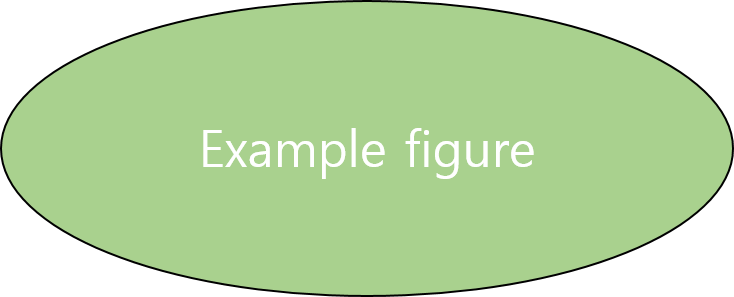
\includegraphics[scale=.35]{./fig/fig_example}
\caption{문제 설명 그림} \label{f-1}
\end{figure}
 

\newpage
\section{연구 동기 및 공헌}\label{s1.2}
본 연구의 동기 및 공헌은 다음과 같다.
\begin{enumerate}
\item[(a)] 연구된 적 없는 생산 계획 문제를 소개한다.
\item[(b)] 최적화 기법에 기반한 다양한 해법을 제안한다.
\item[(c)] 제안한 해법의 효과를 입증하기 위해 다양한 인스턴스에 대한 실험을 진행한다.
\end{enumerate}

\newpage
\section{논문구성}\label{s1.3}
본 논문은 5 장으로 구성된다. 제 \ref{c2}장에서는 선행 연구를 살펴본다. 제 \ref{c3}장에서는 다양한 해법을 제안한다. 제 \ref{c4}장에서는 실험 결과를 살펴본다. 마지막으로 제 \ref{c5}장에서는 결론과 향후 연구방향을 제시한다.

\chapter{선행연구}\label{c2}
\section{생산 계획 문제에 대한 선행 연구}\label{s2.1}
생산 계획 문제를 풀기 위해 다양한 연구가 진행되어 왔다. (예를 들어, \cite{bertsimas1997introduction, gicquel2008mip, jans2008modeling,wolsey1998integer}를 참조). 우리는 Duarte 등 \cite{duarte2013discrete}이 제안한 해법을 확장시킨다.


\newpage
\chapter{해법}\label{c3}
\section{최적화 해법}\label{s3.1}
 총 비용 $f_0(x)$은 고정비용 $fc(x)$과 가변비용 $vc(x)$의 합이다. 즉, 다음의 식이 성립한다.
\begin{equation}
f_0(x)=fc(x)+vc(x)
\end{equation}

문제를 다음과 같이 모형화할 수 있다.
\begin{align}
\text{minimize} \qquad &f_0(x) \label{e1} \\
\text{subject to} \qquad &f_i(x)\leq 0 &\forall i \in I \label{e2}\\
&g_j(x)=0 &\forall j \in J \label{e3}\\
&x\in \mathbb{X} \label{e4}
\end{align}
(\ref{e1})은 목적함수이다. (\ref{e2})과 (\ref{e3})는 제약식이다. 변수의 정의역은 (\ref{e4})를 통해 정의된다.
\begin{proposition}\label{p3.1}\setstretch{1.5}
(\ref{e1})-(\ref{e4})를 다항시간 내에 풀 수 있다..  
\begin{proof}
 $f_0, f_i ,g_j$가 선형이고 $\mathbb{X}$ 이 다면체이므로 선형계획 문제이며 선형계획 문제에 대한 다항시간 알고리즘이 존재한다.
\end{proof}
\end{proposition}
\newpage
\section{휴리스틱 알고리즘}\label{s3.2}
제안된 휴리스틱 알고리즘의 pseudo-code는 아래와 같다.
\begin{algorithm}[h]
\begin{algorithmic}

\State $\mathcal{RP} \leftarrow$ LP relaxation of $\mathcal{P}$, 
\State $n \leftarrow 0;$
\While{$nl+r \leq |T|$}
 \ForAll{$i \in I$, $t \in [nl, nl+r]$}
  \State declare $x_{it} \in \{0,1\}$ in $\mathcal{RP}$;
 %\EndFor
 \EndFor
 \State solve $\mathcal{RP}$ and get solution $(\bar{x})$;
 \ForAll{$i \in I$, $t \in [nl, (n+1)l]$}
  \If{$\overline{x}_{it}=1$}
  \State fix $x_{it} = \overline{x}_{it}$
  \EndIf
 \EndFor
 \State $n\leftarrow n+1;$
\EndWhile \\
\Return feasible solution for $\mathcal{P}$;
\caption{Heuristic Algorithm ($\mathcal{P},r,l$)}
\end{algorithmic}
\end{algorithm}\label{heuristic algorithm}

\chapter{실험 결과}\label{c4}
\section{실험 문제}
실험에 사용된 문제에 대한 설명이 표 \ref{tb1}에 제시되어 있다.

\begin{table}[h]
\centering
\caption{실험 인스턴스 설명}
\begin{tabular}{c||c|c|c}
\toprule
Set& Fixed Cost& Variable Cost & Demand level\\
\hline
I &	\multirow{2}{*}{0}	&\multirow{2}{*}{0}	&low\\
\cline{4-4}
 II& & &high\\
\hline
III &	\multirow{2}{*}{$DU(fc^{min},fc^{max})$}&	\multirow{2}{*}{$DU(vc^{min},vc^{max})$} &low\\
\cline{4-4}
IV &&&high\\
\bottomrule
\end{tabular}
\label{tb1}
\end{table}


\newpage
\section{실험 결과}
실험 진행을 위해 상용 소프트웨어 \cite{xpress}를 사용하였다. 실험 결과는 표 \ref{tb2}에 제시되어 있다. 이 결과는 제안된 기법이 (\textit{New}) 기존의 기법 (\textit{Old})에 비해 효과가 좋다는 사실을 입증한다. 

\begin{table}[h]
\centering
\begin{footnotesize}
\caption{실험 결과}
\begin{tabular}{@{}cc||cc|cc|cc@{}}
\toprule
\multirow{2}{*}{\textit{Dim}} & \multirow{2}{*}{\textit{Set}}  & \multicolumn{2}{c|}{$Gap$} & \multicolumn{2}{c|}{\textit{Time}}& \multicolumn{2}{c}{\#$Opt$/\#$Feas$}\\
&& \textit{Old} & \textit{New}& \textit{Old} & \textit{New}& \textit{Old} & \textit{New}\\
\hline
\multirow{4}{*}{$30\times30$} & I& 61.11 	&3.41 	&0.94 	&0.07 	&10/10	&10/10\\
& II&	17.21 	&0.23  		&0.90 	&0.05 	&10/10	&10/10\\
& III&	48.62 	&8.17  	 	&0.94 	&0.18 	&10/10	&10/10\\
& IV&	15.46 	&0.28 		&0.79 	&0.09 	&10/10	&10/10\\
\hline
\multirow{4}{*}{$100\times 100$} & I&85.75 	&5.24 		&559.19 	&9.71 	&2/10	&10/10\\
&II&9.87 	&0.53 		&394.92 	&2.82 	&8/10	&10/10\\
&III&77.11 	&61.47  	&600 	&600 	&0/3	&6/10\\
&IV&20.71 	&10.47	&496.36 	&409.06 	&0/5	&5/10\\
\bottomrule
\end{tabular}
\label{tb2}
\end{footnotesize}
\end{table}

\chapter{결론}\label{c5}
\section{결론}\label{s5.1}
본 논문에서는 생산 계획 문제를 풀기 위한 최적화 기법을 제안하였다.
\section{향후 연구}\label{s5.2}
제안된 기법을 일반화 시켜 다른 문제에도 적용할 수 있다.



\begin{bibpage}
\bibliography{ref-example}
\bibliographystyle{siam} % Or any other style you like
\nocite{*}
\end{bibpage}

\keywordalt{Production planning, Optimization, Industrial engineering}
\begin{abstractalt}
In this thesis, we consider a production planning problem arising in real-world industry. We propose mathematical optimization techniques for solving the problem. We verify that the proposed solution approaches are more effective than existing methods.
\end{abstractalt}

\acknowledgement\setstretch{1.6}
서울대학교 산업공학과의 모든 식구들께 감사드립니다.
\end{document}

